\section{Objective ablation on MOSTA}
\label{app:objective-ablation}

We compare No Cross, CS, and ZoomST using a common initialization, the same training data and training budget, and identical training settings apart from the loss terms. No Cross uses within-granularity learning; CS adds coarse-support supervision; ZoomST further adds JointMMD. Evaluation uses frozen encoders and the held-out MOSTA split from Section~\ref{sec:developmental-information}, with identical evaluation observations and readout settings across the three models. All readouts use Joint representations at granularities 8, 32, and 128.

Table~\ref{tab:mosta-objective-ablation} follows the anatomical clustering, Brain developmental ordering, and stage-prediction protocols in Appendix~\ref{app:dual-view}--\ref{app:developmental-ordering}.

Adding JointMMD to CS reduces stage-prediction MAE and increases spot-level DPT correlation at all three granularities, with the largest gains at granularity 128. AMI increases at granularities 8 and 32 and remains similar at granularity 128.

\begin{table}[!htbp]
\centering
\caption{\textbf{Controlled objective ablation on MOSTA.} Joint AMI, Brain spot-level DPT--stage Spearman correlation, and Brain stage-prediction MAE. AMI averages the eight held-out sections equally; $\pm$ denotes SD over downstream clustering runs. DPT and stage MAE use the protocols and aggregation of Table~\ref{tab:cross-granularity-development}b. Bold marks the best unrounded mean in each column.}
\label{tab:mosta-objective-ablation}
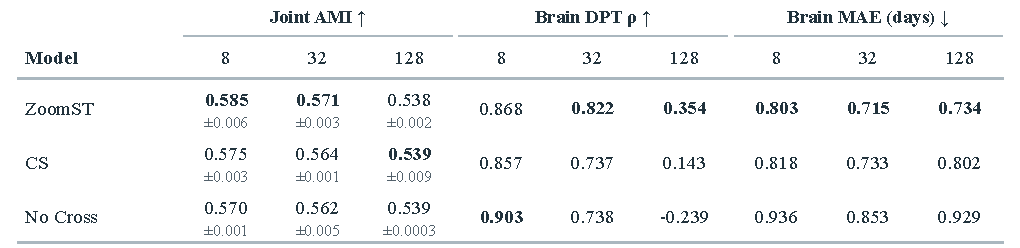
\includegraphics[width=\linewidth]{figures/mosta_objective_ablation.pdf}
\end{table}
\FloatBarrier
